\documentclass{article}
\usepackage[margin=2.5cm]{geometry}
\usepackage{graphicx}
\usepackage{float}
\usepackage{hyperref}
\hypersetup{
    colorlinks=true,
    linkcolor=blue,
    filecolor=magenta,      
    urlcolor=cyan,
    pdftitle={Overleaf Example},
    pdfpagemode=FullScreen,
    }

\title{Report for the Course Bildverarbeitung 103-0274-01L FS22}
\author{Daniel Pfister}
\date{\today}
\graphicspath{{../images/}  {../results/} {../inputs/}}

\begin{document}
    \maketitle
    \section{Fouriertransformation}

    \subsection{Transformation}
    Figure 1 shows the input image on the left and the spectrum after applying \verb|scipy.fft.fft2| and shifting it using \verb|scipy.fft.fftshift|.
    \begin{figure}[H]
        \centering
        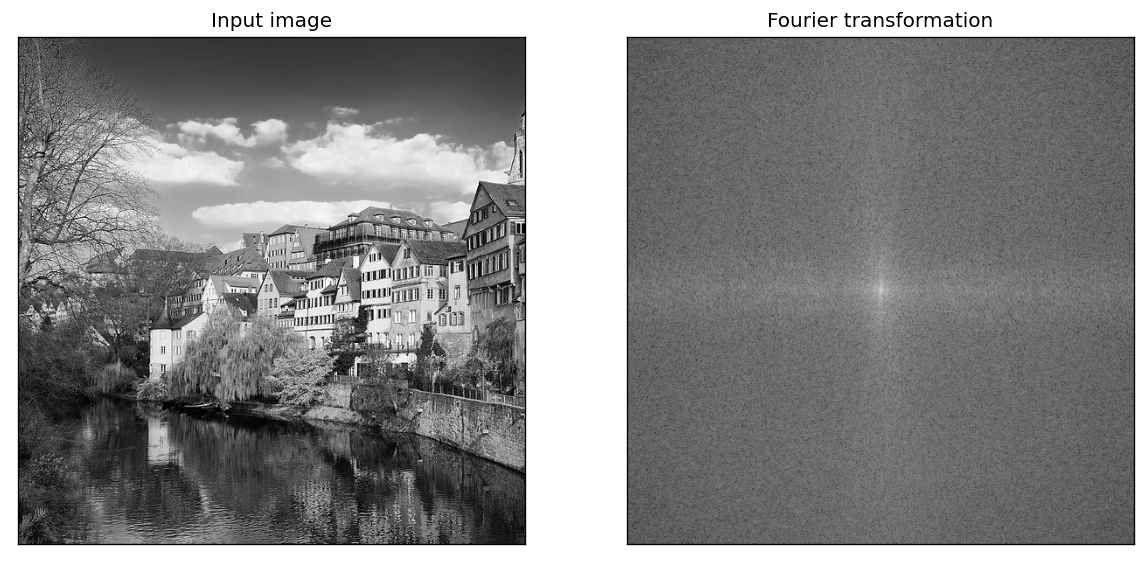
\includegraphics[width = 0.65\textwidth]{fft_1}
        \caption{the input image shown in image and fourier space}
        \label{fig:fft_1}
    \end{figure}

    \subsection{High-pass filter}
    For this task a perfect high-pass filter was constructed and applied in Fourier space.
    Afterwards the spectrum was transformed back into image space using \verb|scipy.fft.ifft2|
    \begin{figure}[H]
        \centering
        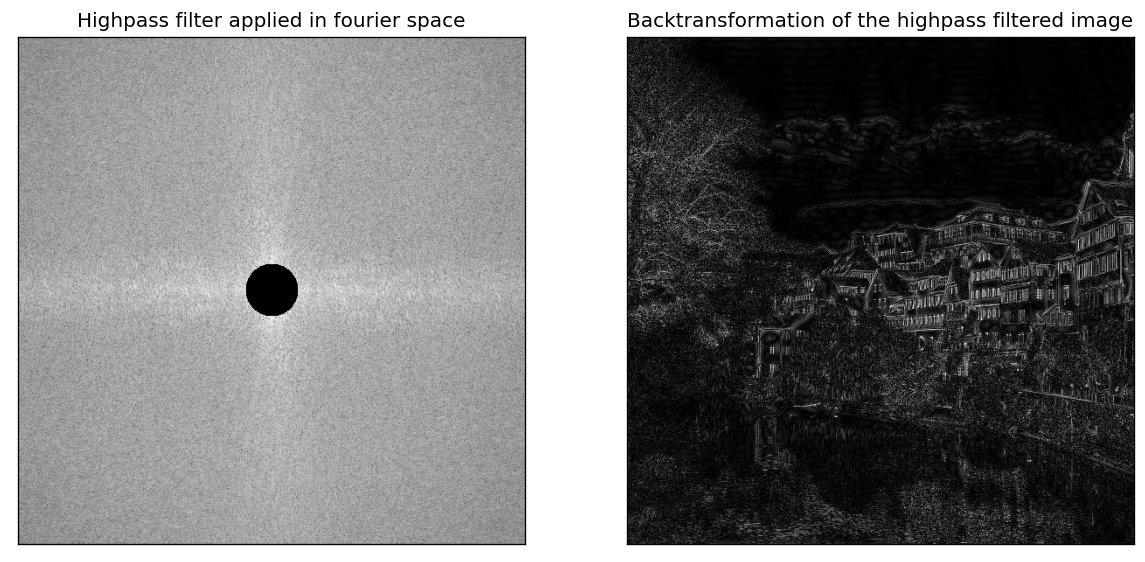
\includegraphics[width = 0.65\textwidth]{highpassfilter.png}
        \caption{the image after applying a high-pass filter shown in fourier and image space}
        \label{fig:highpassfilter}
    \end{figure}

    \subsection{Gaussian filter}
    In this task a Gaussian filter was first constructed in the image space and applied to the image by applying a convolution.
    Afterwards the filter was transformed to the Fourier space using \verb|scipy.fft.fft2| and applied to the spectrum of the image using multiplication.
    Additionally, the average numerical difference between the pixel values of the two results was calculated to be 0.073

    \begin{figure}[H]
        \centering
        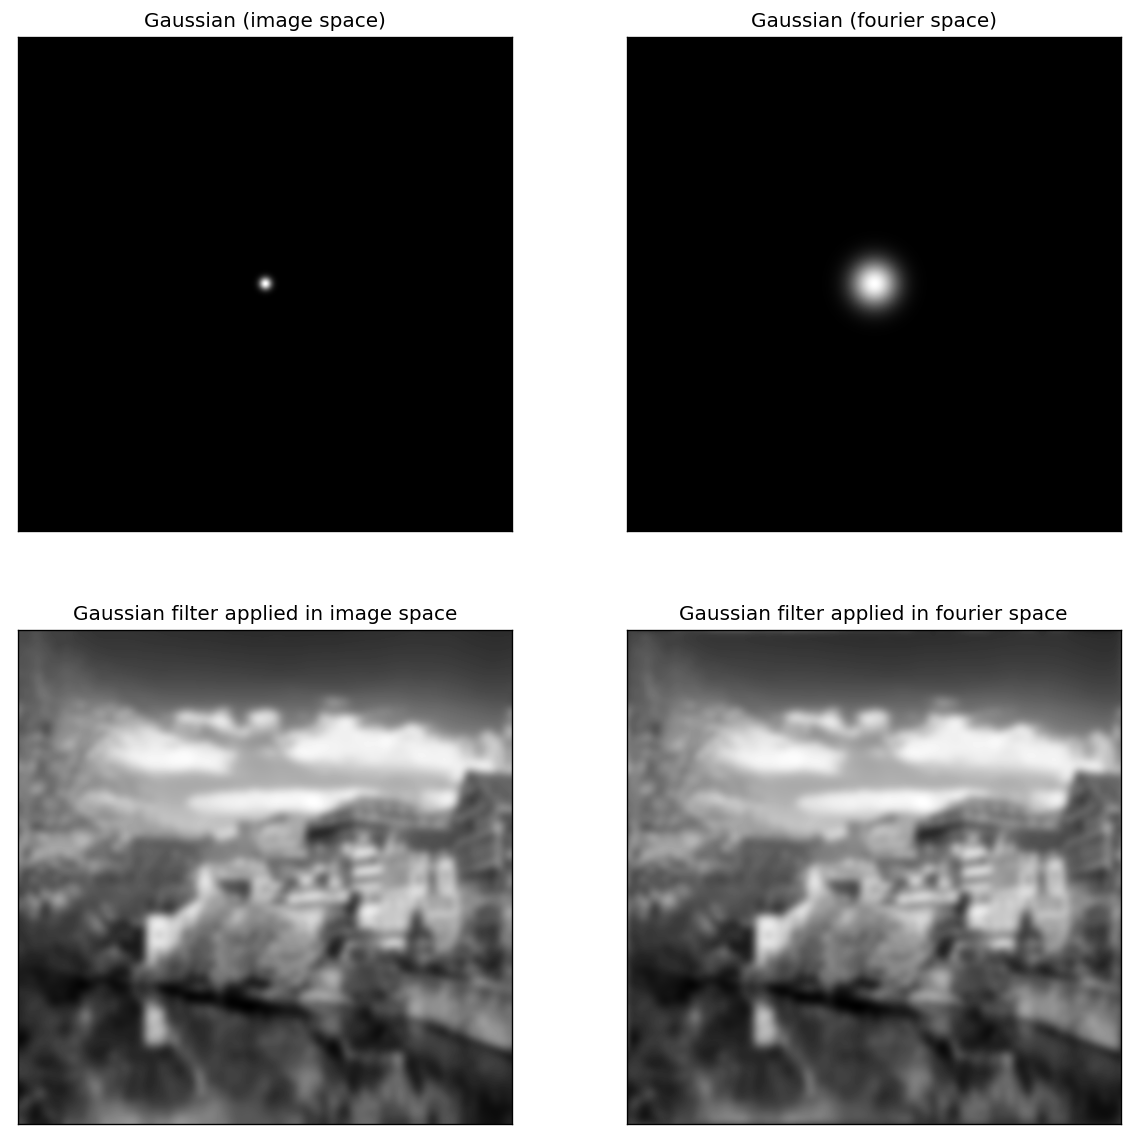
\includegraphics[width = 0.65\textwidth]{gaussian.png}
        \caption{the Gaussian filter in image and fourier space and the images after applying the filter}
        \label{fig:gaussianfilter}
    \end{figure}

    \subsubsection*{1.3.6 Computational Difference}
    The Gaussian filter can either be applied in x and y direction simultaneously using a 2d kernel,
    or it can be applied seperately for each direction, using a 1d kernel each. The result stays the same.
    Here, the computational difference between the two methods was explored, by looping each method 20 times and calculating the mean time.
    The average computation time of the 2d application of the Gaussian filter was measured to be 653.27ms, while the average measured time using the seperate 1d application was 38.13ms.


    \pagebreak

    \section{Morphology}

    \subsection{Coins}

    This is the original image of the coins:

    \begin{figure}[H]
        \centering
        \includegraphics[width = 0.35\textwidth]{coins.jpg}
        \caption{original image of coins}
        \label{fig:coins_original}
    \end{figure}

    \subsubsection{Segmentation}

    The coins were seperated from the background by transforming the RGB image into HSV image space,
    where the saturation corresponds to how "colorful" a pixel is. A mask was created at the places where the saturation was in the range of $[0, 25]$.
    These were the background pixels and they were set to black to create the resulting image.

    \begin{figure}[H]
        \centering
        
\includegraphics[width = 0.35\textwidth]{coins_seg.png}
        \caption{the segemented image of the coins}
        \label{img:coins_segmented}
    \end{figure}

    \subsubsection{Closing Holes}

    The segmented image with the holes within the coins was given. To close the holes,
    the image was first dilated and then eroded.

    \begin{figure}[H]
        \centering
        
\includegraphics[width = 0.35\textwidth]{coins_close.png}
        \caption{image of the coins after closing the holes}
        \label{img:coins_close}
    \end{figure}

    \subsubsection{Instance Segmentation}

    For this task, first the result from the previous image was thresholded to create a binary image. Afterwards the distance transform was applied
    and the certain foreground and certain background were definied using dilation and erosion.
    Then, markers were placed on each certain foreground instance and the watershed algorithm was applied. In the last step,
    each new marker was colored with a random color.

    \begin{figure}[H]
        \centering
        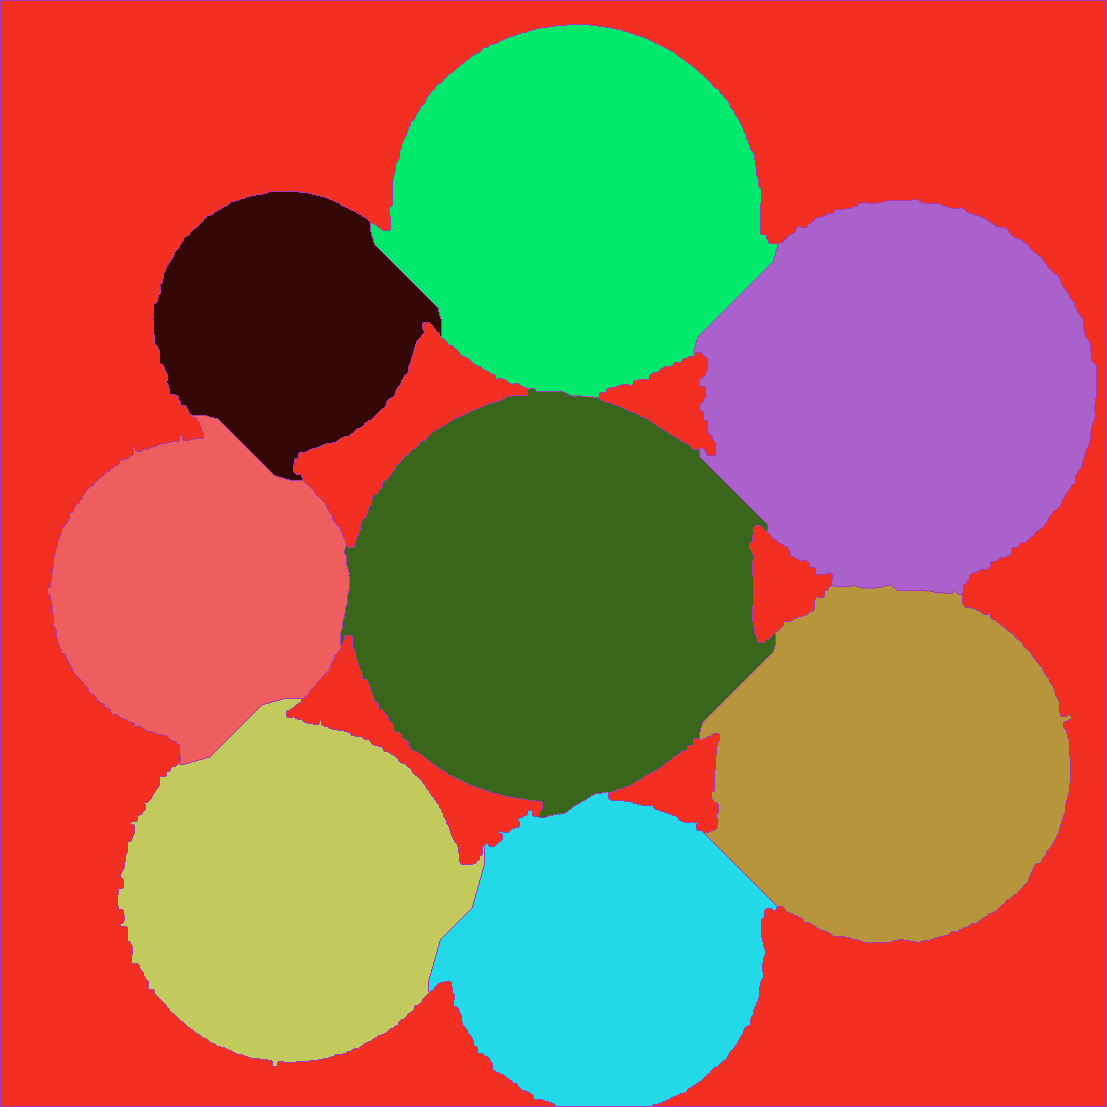
\includegraphics[width = 0.35\textwidth]{coins_instances.png}
        \caption{image of the coins after applying the watershed algorithm}
        \label{img:coins_instances}
    \end{figure}

    \pagebreak

    \subsection{Letter Recognition}

    Here, the image of the text and the image of letter were first transformed into a binary image,
    using \verb|cv.THRESH_BINARY_INV| or \verb|cv.THRESH_BINARY|, respectively. Afterwards the binary image of the text was eroded with the binary image of the letter as kernel to find the instances of the letter.
    Finally, the image was dilated back to have an image constructed of m's.

    \begin{figure}[H]
        \centering
        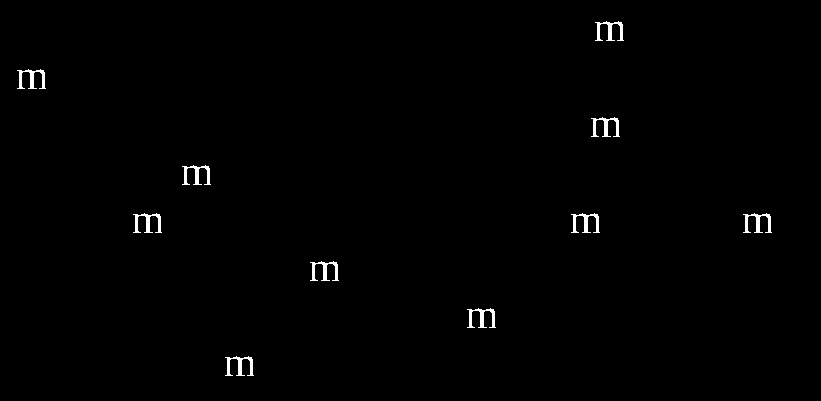
\includegraphics[width = 0.35\textwidth]{text_recog_results.png}
        \caption{result of finding the letters in the image}
        \label{img:text_recog}
    \end{figure}

    \pagebreak

    \section{Corner Detector}

    In the task the Shi-Tomasi and Harris corner detectors were implemented. For the Harris response, first the gradient along x and y was calculated using a Sobel kernel.
    Afterwards the structure tensor and the response were calculated and plotted.

    \begin{figure}[H]
        \centering
        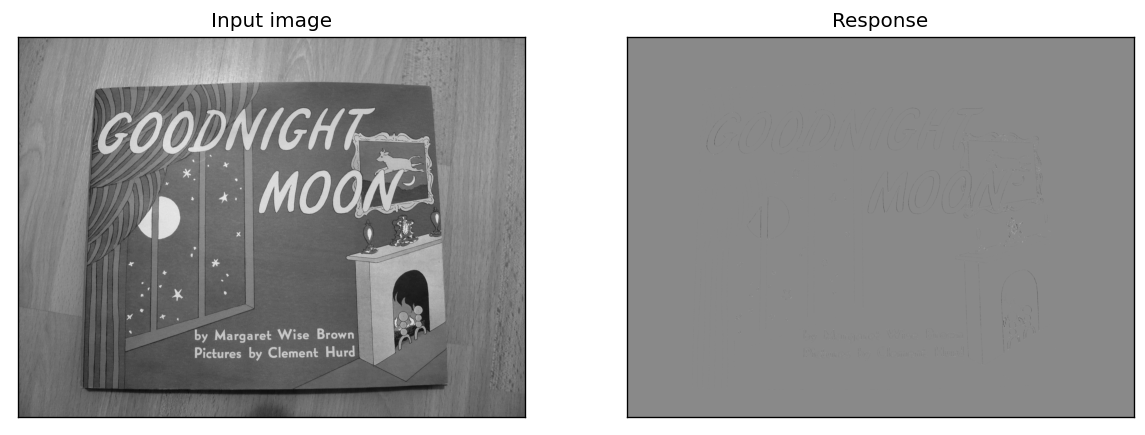
\includegraphics[width = 0.65\textwidth]{harris_response.png}
        \caption{Harris response of the input image}
        \label{img:harris_response}
    \end{figure}

    Then the response was thresholded and a red circle was placed at every valid pixel.

    \begin{figure}[H]
        \centering
        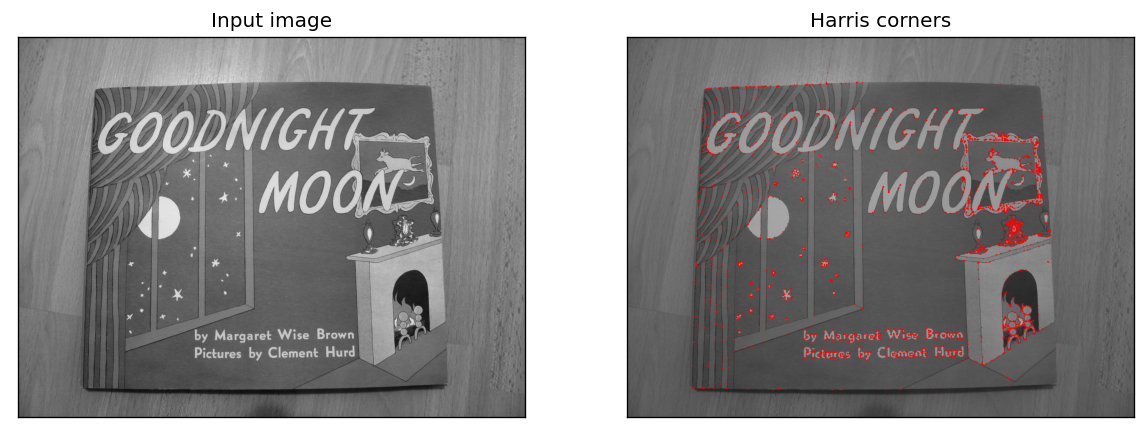
\includegraphics[width = 0.65\textwidth]{harris_before.png}
        \caption{Harris corner detection}
        \label{img:harris_before}
    \end{figure}    

    Finally, \verb|scipy.ndimage.maximum_filter| was applied to get the local maxima of the corners.

    \begin{figure}[H]
        \centering
        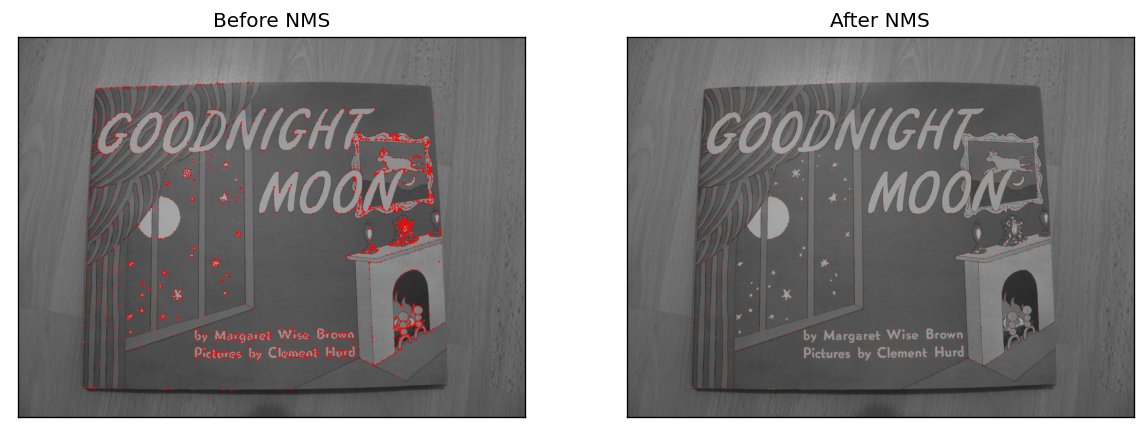
\includegraphics[width = 0.65\textwidth]{harris_after.png}
        \caption{Harris corner detection after NMS}
        \label{img:harris_after}
    \end{figure}

    For the rotated image, the results look the same, because the only difference is that the x and y dimensions were swapped.
    Below are the three results for the rotated image.

    \begin{figure}[H]
        \centering
        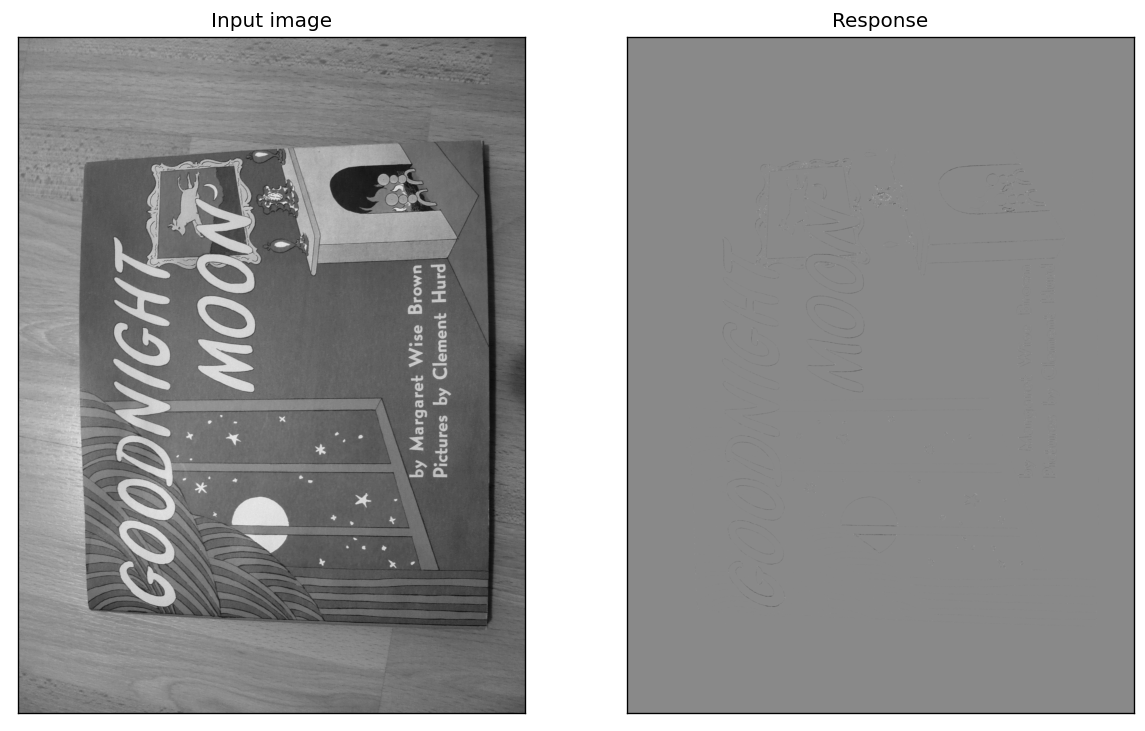
\includegraphics[width = 0.45\textwidth]{harris_response_rotated.png}
        \caption{Harris response of the input image (rotated)}
        \label{img:harris_response_rotated}
    \end{figure}

    \begin{figure}[H]
        \centering
        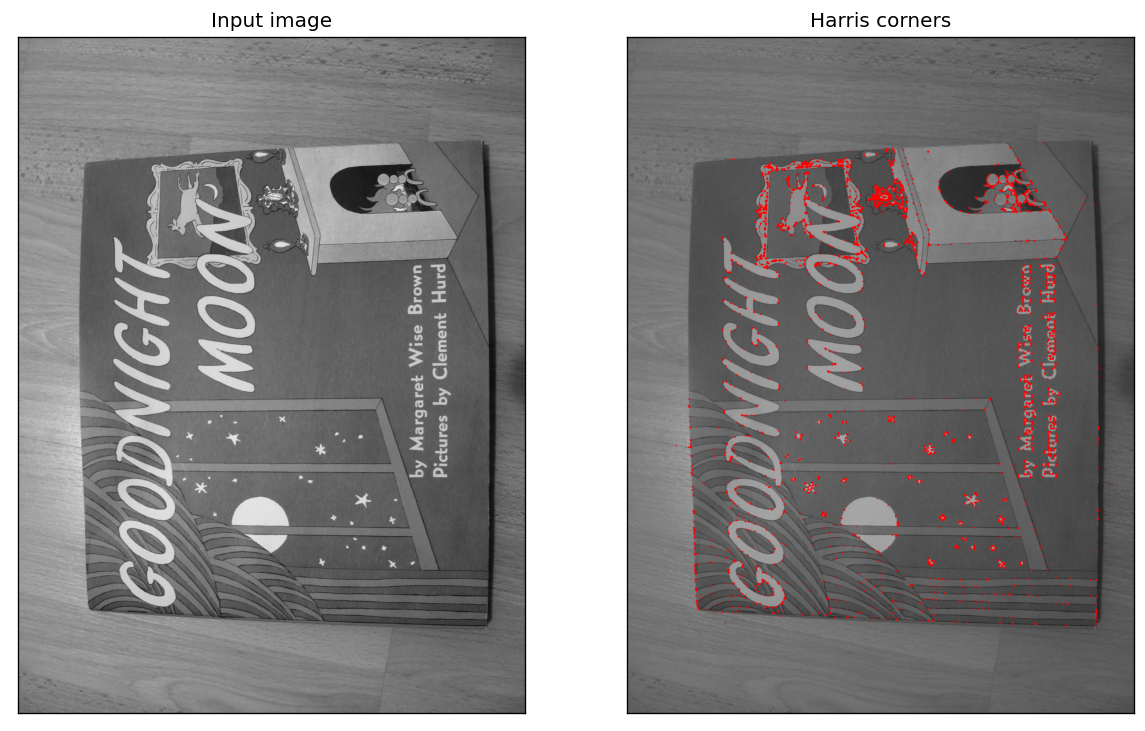
\includegraphics[width = 0.45\textwidth]{harris_before_rotated.png}
        \caption{Harris corner detection (rotated)}
        \label{img:harris_before_rotated}
    \end{figure}   

    \begin{figure}[H]
        \centering
        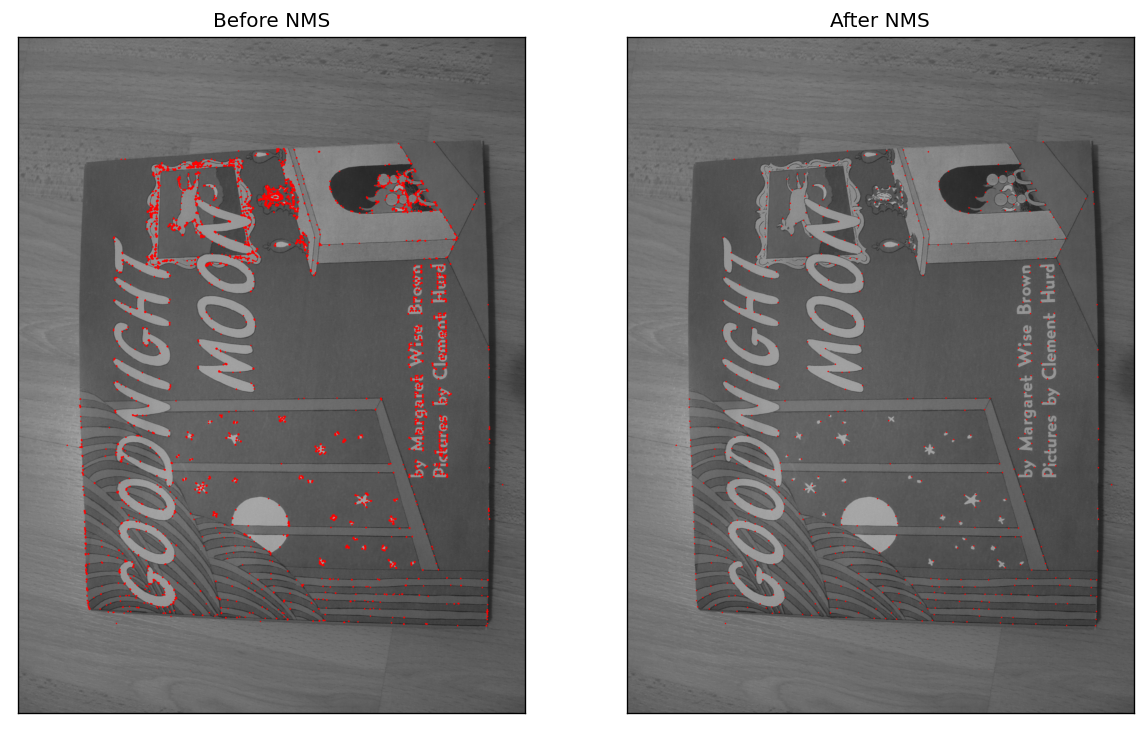
\includegraphics[width = 0.45\textwidth]{harris_after_rotated.png}
        \caption{Harris corner detection after NMS (rotated)}
        \label{img:harris_after_rotated}
    \end{figure}

    \pagebreak

    \section{Canny Edge Detection}

    Here, the image was first blurred by applying a Gaussian filter.

    \begin{figure}[H]
        \centering
        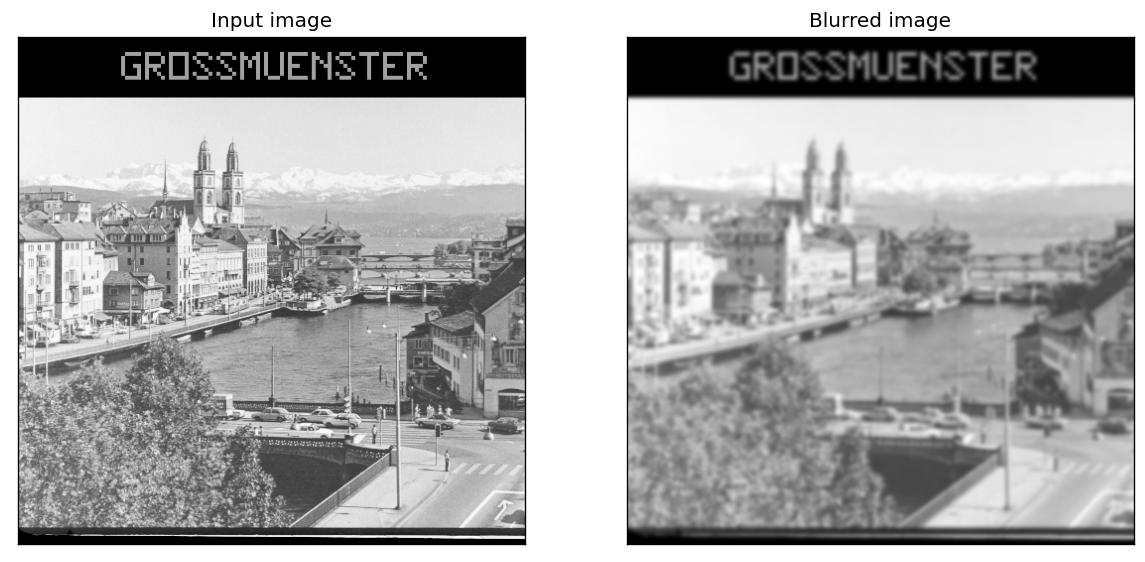
\includegraphics[width = 0.45\textwidth]{canny_blur.png}
        \caption{Image after applying Gaussian blur}
        \label{img:canny_blur}
    \end{figure}

    Afterwards the gradient was calculated by convolving the image with a Sobel kernel.
    Using those gradients the magnitude and direction was found and plotted.

    \begin{figure}[H]
        \centering
        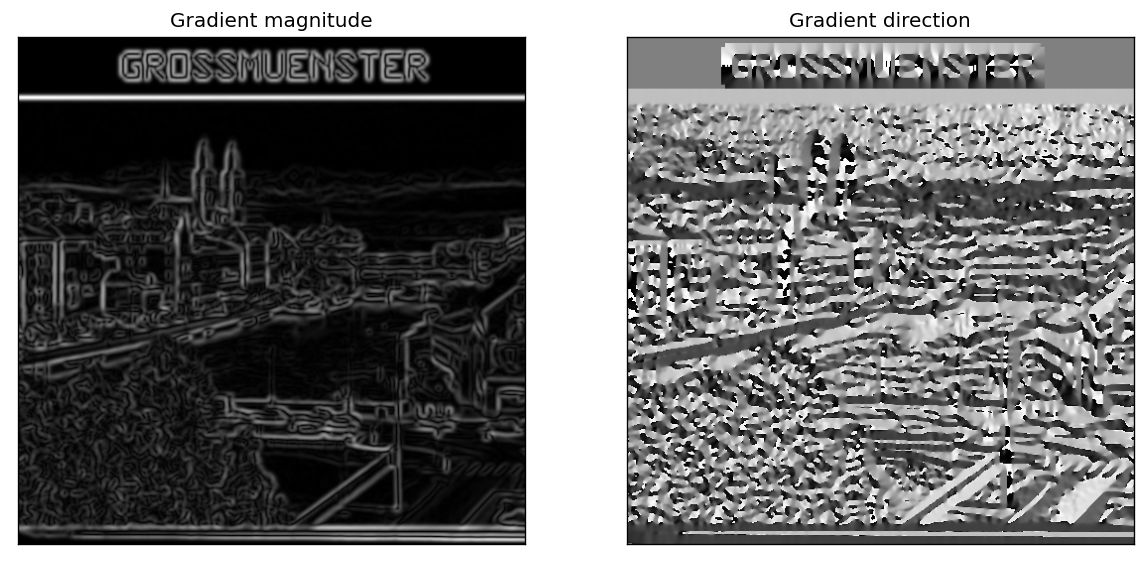
\includegraphics[width = 0.45\textwidth]{canny_magdir.png}
        \caption{Magnitude and Direction of the blurred image}
        \label{img:canny_magdir}
    \end{figure}

    Finally, the NMS seen in the lecture was applied using code from \href{https://github.com/FienSoP/canny_edge_detector}{Github} and visualized.

    \begin{figure}[H]
        \centering
        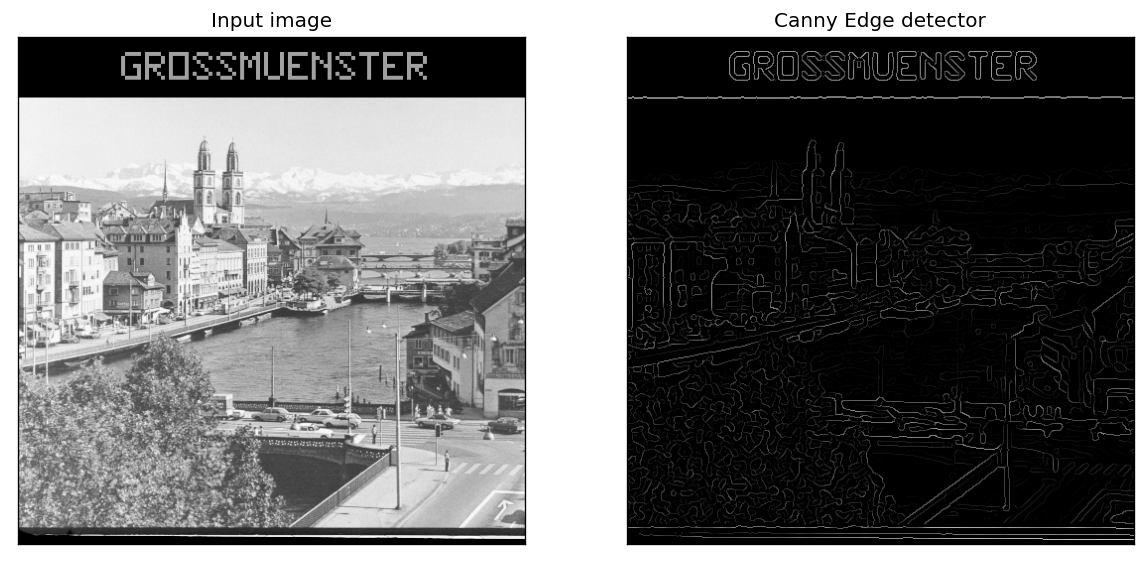
\includegraphics[width = 0.45\textwidth]{canny_nms.png}
        \caption{Canny Edge Detection after applying NMS}
        \label{img:canny_nms}
    \end{figure}

    \subsection{Final Words}

    The code and result images can be found on my personal \href{https://github.com/danpfister/Bildverarbeitung-FS2022}{Github}.

\end{document}